\documentclass[14pt]{extbook}
\usepackage{multicol, enumerate, enumitem, hyperref, color, soul, setspace, parskip, fancyhdr} %General Packages
\usepackage{amssymb, amsthm, amsmath, bbm, latexsym, units, mathtools} %Math Packages
\everymath{\displaystyle} %All math in Display Style
% Packages with additional options
\usepackage[headsep=0.5cm,headheight=12pt, left=1 in,right= 1 in,top= 1 in,bottom= 1 in]{geometry}
\usepackage[usenames,dvipsnames]{xcolor}
\usepackage{dashrule}  % Package to use the command below to create lines between items
\newcommand{\litem}[1]{\item#1\hspace*{-1cm}\rule{\textwidth}{0.4pt}}
\pagestyle{fancy}
\lhead{Progress Quiz 10}
\chead{}
\rhead{Version B}
\lfoot{6232-9639}
\cfoot{}
\rfoot{Fall 2020}
\begin{document}

\begin{enumerate}
\litem{
Describe the end behavior of the polynomial below.\[ f(x) = -6(x + 5)^{2}(x - 5)^{5}(x + 6)^{5}(x - 6)^{5} \]\begin{enumerate}[label=\Alph*.]
\begin{multicols}{2}\item 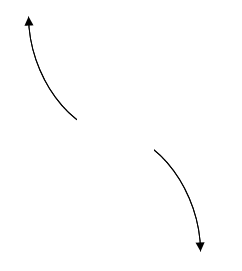
\includegraphics[width = 0.3\textwidth]{../Figures/polyEndBehaviorAB.png}\item 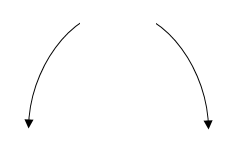
\includegraphics[width = 0.3\textwidth]{../Figures/polyEndBehaviorBB.png}\item 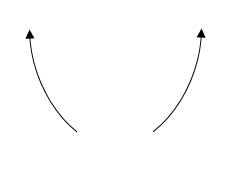
\includegraphics[width = 0.3\textwidth]{../Figures/polyEndBehaviorCB.png}\item 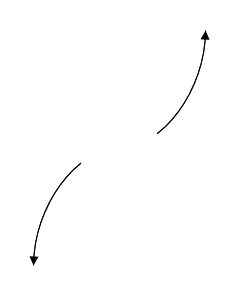
\includegraphics[width = 0.3\textwidth]{../Figures/polyEndBehaviorDB.png}\end{multicols}\item None of the above.
\end{enumerate} }
\litem{
Construct the lowest-degree polynomial given the zeros below. Then, choose the intervals that contain the coefficients of the polynomial in the form $x^3+bx^2+cx+d$.\[ 3 - 5 i \text{ and } -1 \]\begin{enumerate}[label=\Alph*.]
\item \( b \in [0, 3.1], c \in [-11, 2], \text{ and } d \in [-8, 1] \)
\item \( b \in [1.1, 5.6], c \in [20, 29], \text{ and } d \in [-35, -31] \)
\item \( b \in [-5.2, -3], c \in [20, 29], \text{ and } d \in [31, 38] \)
\item \( b \in [0, 3.1], c \in [1, 9], \text{ and } d \in [0, 8] \)
\item \( \text{None of the above.} \)

\end{enumerate} }
\litem{
Describe the zero behavior of the zero $x = 9$ of the polynomial below.\[ f(x) = 8(x + 9)^{5}(x - 9)^{10}(x - 8)^{8}(x + 8)^{12} \]\begin{enumerate}[label=\Alph*.]
\begin{multicols}{2}\item 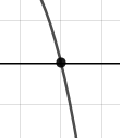
\includegraphics[width = 0.3\textwidth]{../Figures/polyZeroBehaviorCopyAB.png}\item 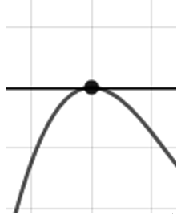
\includegraphics[width = 0.3\textwidth]{../Figures/polyZeroBehaviorCopyBB.png}\item 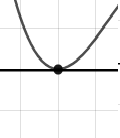
\includegraphics[width = 0.3\textwidth]{../Figures/polyZeroBehaviorCopyCB.png}\item 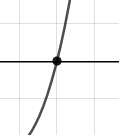
\includegraphics[width = 0.3\textwidth]{../Figures/polyZeroBehaviorCopyDB.png}\end{multicols}\item None of the above.
\end{enumerate} }
\litem{
Construct the lowest-degree polynomial given the zeros below. Then, choose the intervals that contain the coefficients of the polynomial in the form $ax^3+bx^2+cx+d$.\[ 1, \frac{-3}{4}, \text{ and } \frac{-5}{3} \]\begin{enumerate}[label=\Alph*.]
\item \( a \in [12, 19], b \in [14.9, 17.6], c \in [-25, -7], \text{ and } d \in [10, 23] \)
\item \( a \in [12, 19], b \in [22.9, 25], c \in [-9, -3], \text{ and } d \in [-15, -12] \)
\item \( a \in [12, 19], b \in [-19.1, -15.4], c \in [-25, -7], \text{ and } d \in [10, 23] \)
\item \( a \in [12, 19], b \in [14.9, 17.6], c \in [-25, -7], \text{ and } d \in [-15, -12] \)
\item \( a \in [12, 19], b \in [40.2, 44], c \in [38, 47], \text{ and } d \in [10, 23] \)

\end{enumerate} }
\litem{
Which of the following equations \textit{could} be of the graph presented below?
\begin{center}
    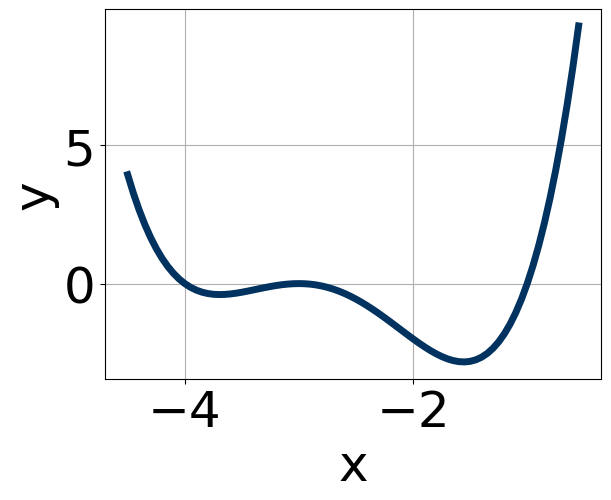
\includegraphics[width=0.5\textwidth]{../Figures/polyGraphToFunctionB.png}
\end{center}
\begin{enumerate}[label=\Alph*.]
\item \( 16(x + 3)^{5} (x + 1)^{6} (x + 4)^{11} \)
\item \( 19(x + 3)^{6} (x + 1)^{10} (x + 4)^{7} \)
\item \( 2(x + 3)^{8} (x + 1)^{7} (x + 4)^{5} \)
\item \( -3(x + 3)^{8} (x + 1)^{9} (x + 4)^{10} \)
\item \( -20(x + 3)^{4} (x + 1)^{11} (x + 4)^{9} \)

\end{enumerate} }
\litem{
Describe the zero behavior of the zero $x = -6$ of the polynomial below.\[ f(x) = 5(x - 6)^{5}(x + 6)^{8}(x - 9)^{9}(x + 9)^{11} \]\begin{enumerate}[label=\Alph*.]
\begin{multicols}{2}\item 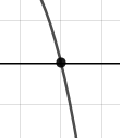
\includegraphics[width = 0.3\textwidth]{../Figures/polyZeroBehaviorAB.png}\item 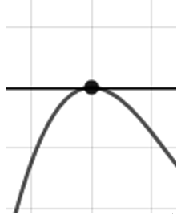
\includegraphics[width = 0.3\textwidth]{../Figures/polyZeroBehaviorBB.png}\item 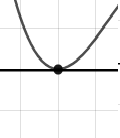
\includegraphics[width = 0.3\textwidth]{../Figures/polyZeroBehaviorCB.png}\item 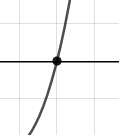
\includegraphics[width = 0.3\textwidth]{../Figures/polyZeroBehaviorDB.png}\end{multicols}\item None of the above.
\end{enumerate} }
\litem{
Describe the end behavior of the polynomial below.\[ f(x) = 2(x + 2)^{2}(x - 2)^{3}(x + 3)^{3}(x - 3)^{5} \]\begin{enumerate}[label=\Alph*.]
\begin{multicols}{2}\item 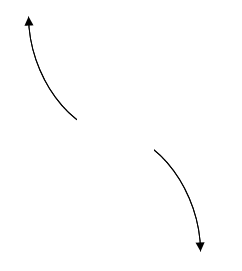
\includegraphics[width = 0.3\textwidth]{../Figures/polyEndBehaviorCopyAB.png}\item 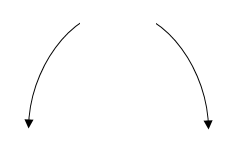
\includegraphics[width = 0.3\textwidth]{../Figures/polyEndBehaviorCopyBB.png}\item 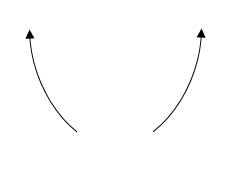
\includegraphics[width = 0.3\textwidth]{../Figures/polyEndBehaviorCopyCB.png}\item 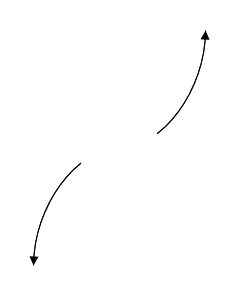
\includegraphics[width = 0.3\textwidth]{../Figures/polyEndBehaviorCopyDB.png}\end{multicols}\item None of the above.
\end{enumerate} }
\litem{
Construct the lowest-degree polynomial given the zeros below. Then, choose the intervals that contain the coefficients of the polynomial in the form $x^3+bx^2+cx+d$.\[ 4 - 3 i \text{ and } 1 \]\begin{enumerate}[label=\Alph*.]
\item \( b \in [-2, 6], c \in [-1, 13], \text{ and } d \in [-5, -1] \)
\item \( b \in [-13, -8], c \in [31, 36], \text{ and } d \in [-26, -23] \)
\item \( b \in [8, 11], c \in [31, 36], \text{ and } d \in [25, 31] \)
\item \( b \in [-2, 6], c \in [-10, -1], \text{ and } d \in [0, 5] \)
\item \( \text{None of the above.} \)

\end{enumerate} }
\litem{
Which of the following equations \textit{could} be of the graph presented below?
\begin{center}
    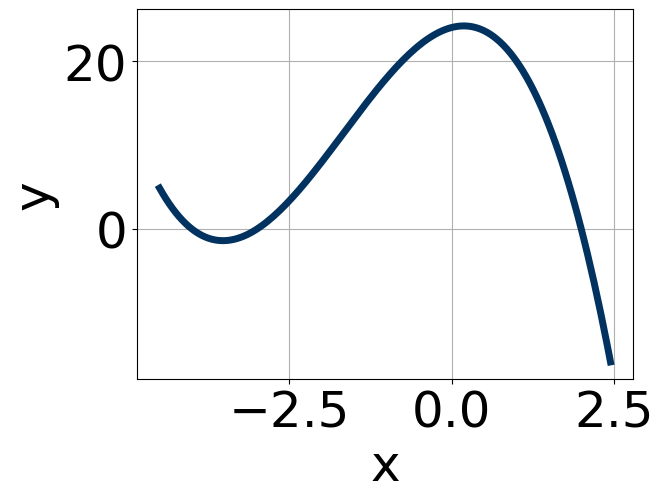
\includegraphics[width=0.5\textwidth]{../Figures/polyGraphToFunctionCopyB.png}
\end{center}
\begin{enumerate}[label=\Alph*.]
\item \( -3(x + 3)^{8} (x + 4)^{6} (x - 2)^{11} \)
\item \( 16(x + 3)^{10} (x + 4)^{11} (x - 2)^{7} \)
\item \( -11(x + 3)^{11} (x + 4)^{9} (x - 2)^{5} \)
\item \( 2(x + 3)^{11} (x + 4)^{11} (x - 2)^{9} \)
\item \( -9(x + 3)^{4} (x + 4)^{7} (x - 2)^{11} \)

\end{enumerate} }
\litem{
Construct the lowest-degree polynomial given the zeros below. Then, choose the intervals that contain the coefficients of the polynomial in the form $ax^3+bx^2+cx+d$.\[ 3, 4, \text{ and } \frac{-1}{2} \]\begin{enumerate}[label=\Alph*.]
\item \( a \in [-4, 5], b \in [14, 19], c \in [26, 35], \text{ and } d \in [7, 17] \)
\item \( a \in [-4, 5], b \in [-21, -10], c \in [11, 26], \text{ and } d \in [-12, -10] \)
\item \( a \in [-4, 5], b \in [-4, 10], c \in [-27, -20], \text{ and } d \in [-12, -10] \)
\item \( a \in [-4, 5], b \in [-21, -10], c \in [11, 26], \text{ and } d \in [7, 17] \)
\item \( a \in [-4, 5], b \in [9, 14], c \in [11, 26], \text{ and } d \in [-12, -10] \)

\end{enumerate} }
\end{enumerate}

\end{document}